\section{Strategi Pengujian: Manual vs Otomatis, Unit vs Integrasi vs End-to-End}

Strategi pengujian menentukan \textit{bagaimana} dan \textit{kapan} pengujian dilakukan. \textbf{Pengujian manual} dilakukan oleh manusia yang berinteraksi langsung dengan aplikasi --- cocok untuk eksplorasi, usabilitas, dan kasus edge. \textbf{Pengujian otomatis} menggunakan skrip yang dijalankan secara berulang --- cocok untuk regresi dan CI/CD. Idealnya, kedua pendekatan dikombinasikan: otomatis untuk pengujian rutin, manual untuk kasus yang sulit diotomasi \cite{mdnToolsTesting}.

Berdasarkan cakupan, pengujian dibagi ke dalam tiga level yang membentuk \textbf{piramida pengujian}: \textbf{unit test} (terbanyak, menguji fungsi/class terisolasi), \textbf{integrasi test} (menguji interaksi antar komponen --- misalnya PHP + database), dan \textbf{end-to-end test} (E2E, paling sedikit, menguji seluruh alur dari perspektif pengguna --- misalnya login $\to$ tambah data $\to$ logout). Semakin tinggi level, semakin lambat dan mahal eksekusinya.

\begin{figure}[ht]
\centering
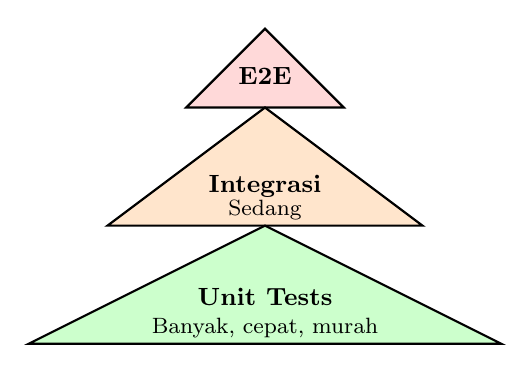
\begin{tikzpicture}
  \fill[green!20] (-3,0) -- (3,0) -- (0,1.5) -- cycle;
  \fill[orange!20] (-2,1.5) -- (2,1.5) -- (0,3) -- cycle;
  \fill[red!15] (-1,3) -- (1,3) -- (0,4) -- cycle;

  \draw[thick] (-3,0) -- (3,0) -- (0,1.5) -- cycle;
  \draw[thick] (-2,1.5) -- (2,1.5) -- (0,3) -- cycle;
  \draw[thick] (-1,3) -- (1,3) -- (0,4) -- cycle;

  \node[font=\small\bfseries] at (0,0.6) {Unit Tests};
  \node[font=\footnotesize] at (0,0.2) {Banyak, cepat, murah};

  \node[font=\small\bfseries] at (0,2) {Integrasi};
  \node[font=\footnotesize] at (0,1.7) {Sedang};

  \node[font=\small\bfseries] at (0,3.4) {E2E};
\end{tikzpicture}
\caption{Piramida pengujian: unit (terbanyak) $\to$ integrasi $\to$ E2E (paling sedikit)}
\end{figure}

\begin{table}[ht]
\centering
\begin{tabular}{|P{2.5cm}|P{5cm}|P{5cm}|}
\hline
\textbf{Aspek} & \textbf{Manual} & \textbf{Otomatis} \\
\hline
Kecepatan & Lambat & Cepat \\
\hline
Konsistensi & Bergantung penguji & Selalu sama \\
\hline
Biaya awal & Rendah & Tinggi (tulis skrip) \\
\hline
Biaya jangka panjang & Tinggi (repetitif) & Rendah (dijalankan ulang) \\
\hline
Cocok untuk & Eksplorasi, usabilitas & Regresi, CI/CD \\
\hline
\end{tabular}
\caption{Perbandingan pengujian manual vs otomatis}
\end{table}

